\section{Mixing time}\label{sec_mix}

Our first experiment will attempt to bound the mixing time of the Hit and Run random walk in a convex shape. The hit and run walk is known to mix rapidly %cite hit and run is fast and fun, as well as Vempala's proof of warm start-ness
in the sense that the number of steps needed for the walk to reach a uniform ditribution is $O^{*}(n^2)$, however this result actually shows that the walk can only be guaranteed to mix after over $10^{10} n^2$
steps. A hit and run step requires the generation of $n$ uniformly distributed random numbers, which is already a difficult task. Performing $10^{10} n^2$ steps, then, is very much infeasible on modern hardware.

We shall judge the walk to be well-mixed if 1,000 independent points generated by the walk with a fixed starting point at the origin pass a $\chi^2$ test at the 1\% level against the null hypothesis that the points are identically distributed to a set of 1,000 points sampled by a method guaranteed to generate uniform points, but which may be somewhat slower. It is not clear which shape is likely to constitute a pathological case for the hit and run walk; the ice cream has the smallest volume, and so in a sense fewer points need to be chosen from, but also has the tighest possible corner, in which the walk is most likely to get stuck. By contrast, the ball has the largest volume and no corners. We will test both shapes. Uniformly distributed random points can be generated from a ball fairly easily, and uniform random points can be generated from an ice cream by simple rejection sampling. To keep our search reasonably short, we will restrict ourselves to only testing numbers of steps equal to natural powers of 2. Due to the extreme scaling of rejection sampling from an ice cream, it is not feasible to test any more than 8 dimensions on a home computer; though the wall clock times are not one of the variables we will be analysing, this information was still gathered for this experiment. If it took $t$ seconds to sample 1,000 points from $n$ dimensions, then it took roughly $10t+t$ to sample the same number of points from $n+1$ dimensions.


We conclude from these tests that, for up to 8 dimensions, using $2^5$ steps produces adequately random points. Whilst there was one exception to this, namely the number of steps to sample from an ice cream where $n=3$, it is also true that a very large number of tests was performed, so it's likely that this one exception is just a statistical outlier.

Given the difficulty of taking a hit and run step, this is still a relatively expensive random number generator, but nowhere near the theoretical upper bound of $10^{10}$. This is relieving, and we will use these 32 steps in the random walk for the following experiments.


\section{Threads per stage}\label{sec_error}

We will now see how the number of threads per phase influences the accuracy of an estimate. In the paper describing our particular estimation method, it is stated that, for an n-dimensional shape, in order to achieve an error of $\varepsilon$, we should use $400\frac{n\log n}{\varepsilon^2}$ threads per stage. This, again, is an upper bound, and we would like to show that it is loose. We shall vary the number of threads used per stage, and see how the distribution of estimates varies with this value. As before, we will use both the ice cream and the ball to respectively maximise and minimise the ratios between successive shapes. Our analysis here will be largely visual, since any returned value from this algorithm might be considered valid for a sufficiently large value of epsilon.

In all cases the errors decrease fairly rapidly, with estimates being easier to acquire for the ball than for the ice cream. The ice cream is very much the pathological case here. These figures can be used to read off the minimum number of threads needed to get an estimate of a given quality, but it is interesting to note that, presumably due to numerical instability, it is impossible to attain an error of 0 in many cases, with estimates showing a clear tendency to converge towards slightly incorrect values. We also depict the greatest errors made on each shape in terms of apsolute error. Because of the vast number of graphs, figure \ref{fig_histograms} we will only show a few.

\begin{figure}
\centering
\subfloat[Histograms for the ball estimates]{
	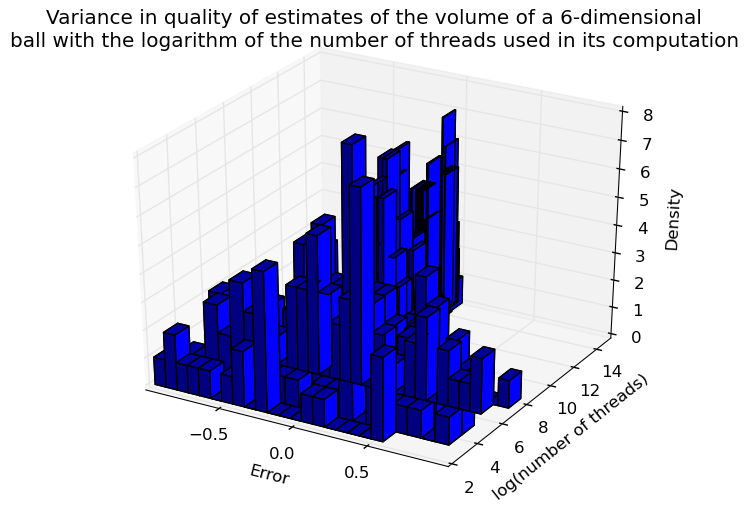
\includegraphics[width = 0.4 \textwidth]{./images/6-dimensions_ball_3d.png}
}
\subfloat[Histograms for the ice cream estimates]{
	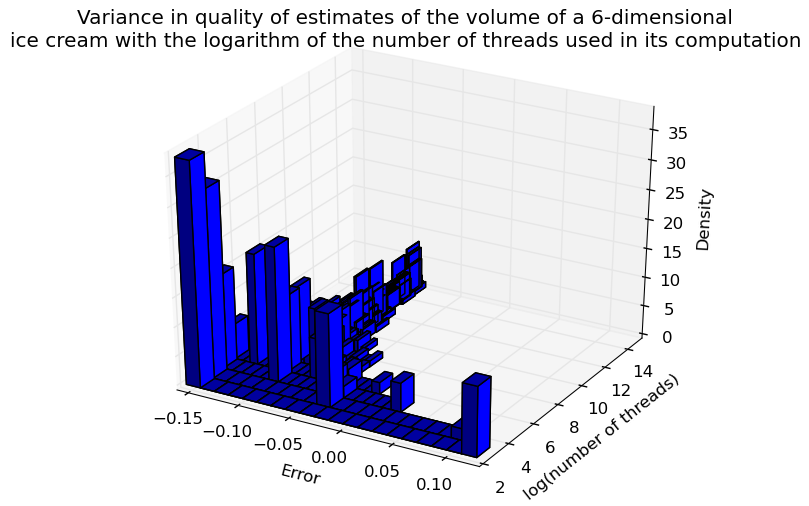
\includegraphics[width = 0.4 \textwidth]{./images/6-dimensions_ice_cream_3d.png}
} 
\\

\subfloat[The worst mistakes made in the ball estimates]{
	\label{fig_2d_ball}
	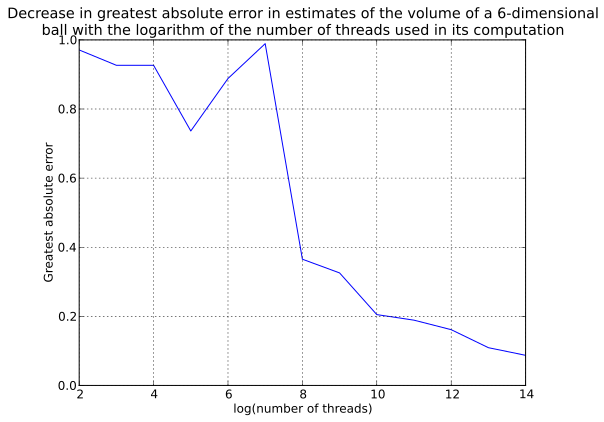
\includegraphics[width = 0.4 \textwidth]{./images/6-dimensions_ball_2d.pdf}
}
\subfloat[The worst mistakes made in the ice cream estimates]{
	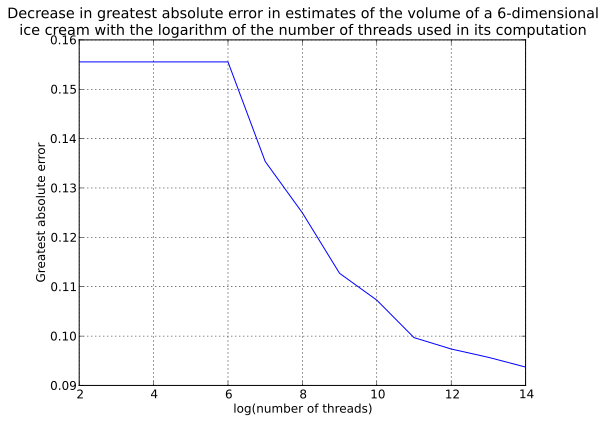
\includegraphics[width = 0.4 \textwidth]{./images/6-dimensions_ice_cream_2d.pdf}
	\label{fig_2d_ice_cream}
}
\label{fig_histograms}
\caption{Variance in errors for various shapes, measured in different ways}
\end{figure}

So, reading off from figures \ref{fig_2d_ice_cream} and \ref{fig_2d_ball}, in a 6-dimensional ice cream our estimates all become correct for $\varepsilon > 0.1$ for any number of threads greater than $2^11 = 2,048$. For a 6-dimensional ball to within an error of $0.1$, we need more like $2^13 = 8,192$. The papers suggest that at least $400\frac{n\log n}{\varepsilon^2} \approxeq 620,000$ threads are necessary for each stage. Once again, the upper bound is very loose indeed.

\section{Computation Time for Convex Shapes}\label{sec_time}

It's now time to test the practicalities of this algorithm on a series of convex shape, against already established methods of exact volume computation. The code used for comparison is the same as that used in %cite exact methods
and was run over a series of randomly generated convex shapes. Each shape is the convex hull of the box $[-1,1]^n$, and some variable number of points on the ball of radius $\sqrt n$. We will randomly generate series of shapes in each dimension, increasing the number of points on the hull, and seeing how this affects the time for a volume estimation to complete to a precision of $\varepsilon = 0.1$.

All experiments were conducted on the same hardware and in the same operating system, using the same time metric. The processor is an Intel i5-2500k in a Gigabyte Z68AP-D3 motherboard, connected to 8 GiB of 1,600 MHz dual-challen DDR3 RAM. The programs were both compiled onto a 64-bit install of Ubuntu 12.04 virtualised by Oracle VM Virtualbox with access to 2GiB of RAM. Each time is measured in elapsed clock cycles divided by the number of clocks per second. Using this processor time removes the possibility of error due to other running processes. Neither program is designed to exploit any more than a single processor core.

The oracle is implemented with a linear programming solver, which tests whether a queried point can be written as a convex combination of the points on a hull. The LP solver used is Gurobi, which is the fastest LP solver currently available.


Unfortunately, despite the high-speed LP solver, the oracle queries are very much not free. The majority of our time in this case is spent answering oracle queries, not performing the auxillary operations. %Talk about scaling of answering oracle queries - if they scale as badly as solving LPs, we're basically wasting our time here. Otherwise, eventually this will be badass